\documentclass[journal]{IEEEtran}
\usepackage{fullpage,enumitem,amsfonts,amsmath,amssymb,graphicx, cite}

\begin{document}
\title{Personal Legal Counselor and Interpreter of the Law via Machine Learning}
\author{Derek Yan, Tianyi Wang, Patrick Chase\\
\{zhyan, tianyiw, pchase\}@stanford.edu}
\markboth{Final report for CS229, Fall 2014}
{Shell \MakeLowercase{\textit{et al.}}: Personal Legal Counselor and Interpreter of the Law via Machine Learning}
\maketitle

\begin{abstract}
The goal of this project was to predict the likelihood of winning a new legal dispute based on results of past cases. We collected over 5000 legal proceedings in the form of case briefs from the internet and used various language processing techniques to parse the raw text into feature vectors. We then used this feature vectors to train several binary classification algorithms, including Naive Bayes, random forests, logistic regression and an SVM. The SVM model achieved the highest test set accuracy of 62\%, which was an improvement over the random 50\% baseline. In this paper, we explain the details of how we transformed the raw text of the case briefs into feature vectors, and how we used them to build several models. We then discuss the results obtained by each of the models and suggest future work that could be done in the area.
\end{abstract}

\begin{keywords}
law, machine learning, case briefs, court cases.
\end{keywords}

\section{Introduction}
\IEEEPARstart{``T} he first thing we do, let?s kill all the lawyers'' - William Shakespeare, 2 Henry VI, 4.2.59. 

Any major transaction, legal procedure, or patent dispute always requires an attorney-at-law in the due process. However, paying an attorney, even for a consultation, can be too expensive and out of reach for much of the population. Due to the exorbitant cost of legal action, many cases are unresolved or dropped. Our goal was to create a tool that would provide legal counsel to people who would otherwise not have access to it. In particular, our model would tell someone the probability they have of winning a given case, which would allow them to make the a better decision of whether or not to pursue further legal action. 

\section{Dataset}

Our dataset was obtained from url{www.casebriefs.com}. It consisted of 5,836 legal case briefs, where each case brief was split up into four segments of text, the \textit{Parties in Dispute}, the \textit{Summary of Facts}, the \textit{Issue of Law}, and the \textit{Verdict}. Fig. \ref{ExampleCaseBrief} is  an example of a very short case brief.

\begin{figure}
    \centering
    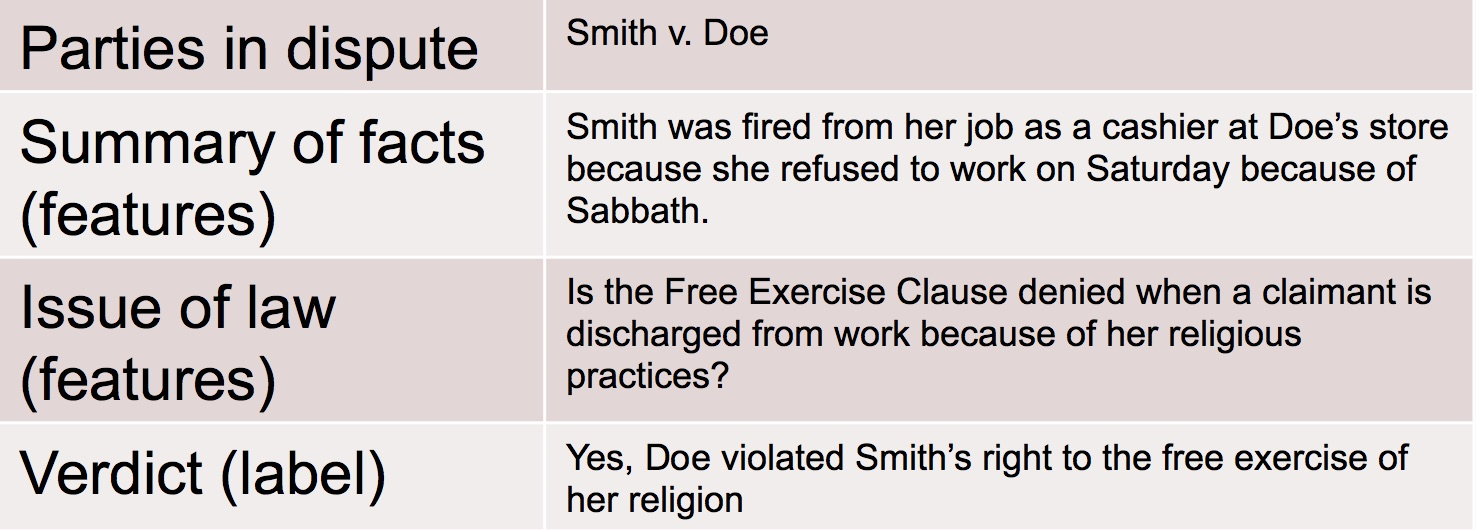
\includegraphics[width=3.5in]{exampleCaseBrief.jpg}
    \caption{Example Case Brief}
    \label{ExampleCaseBrief}
\end{figure}

\section{Features and Preprocessing}

First, we parsed the \textit{Verdict} section to obtain the binary labels for the cases. When the \textit{Verdict} was held, meaning the answer to the \textit{Issue of Law} was "yes," we gave a positive label to the example, but when the answer to the \textit{Issue of Law} was "no" we gave a negative label to the example. 

After extracting the labels, we found that there were 2099 positive cases and 3737 negative cases.

\subsection{Training and Testing Data}

We then split up the data into the training and testing datasets described below.

\begin{table}[ht]
\centering
\begin{tabular}{rrr}
  \hline
& Training Dataset &	Testing Dataset\\
  \hline
Total Examples&	3800&	400 \\
Positive Examples &	1900 &	200 \\
Negative Examples &	1900 &	200 \\
   \hline
\end{tabular}
\end{table}

\subsection{Feature Generation}

To create the feature vectors, we used the \textit{Summary of Facts} section and \textit{Issue of Law} section. We did not use any of the text from the \textit{Verdict} section because that section was used to determine the positive or negative label.

First, we processed the raw text of the case briefs by transforming each word to its stem using the Lancaster Stemmer from the NLTK, Natural Language ToolKit \cite{Loper:2002:NNL:1118108.1118117}. We then formed a dictionary by scanning through all the words in our dataset. After forming the dictionary, we used the dictionary to represent the case briefs using the bag-of-words representation. In our representation, the $i$th element of the feature vector for an example corresponded to the number of times the $i$th stem occurred in the given case brief.

We also experimented with adding bigrams and trigrams to the feature vectors. For the algorithms that took dense matrices as input, this made the input too large and cause the algorithms to take too long or run out of memory. However, the SVM implementation took in a sparse matrix input and this was able to run with bigrams and trigrams.

(Add part of example feature vector?)

\section{Models}

For all the models we used the SciKit-Learn package \cite{scikit-learn} for python.

\subsection{Naive Bayes}

Details.

\subsection{Random Forests}

Details.

\subsection{Logistic Regression}

Details on regularization.

\subsection{SVM}

Details on SVM.

\section{Results}

Large table of results and confusion matrices.

Important words/phrases

\section{Discussion}

\section{Conclusions}



\section{Future Work}



\bibliographystyle{abbrv}
\bibliography{cs229report.bib}

\end{document}

